\section{VPN Based Mobile Measurement Platform} 
\label{sec:platform} 
In this section, we enumerate the goals of a mobile measurement platform,
show how VPNs can be used to achieve the described goals, and finally
present empirical results that demonstrate the feasibility of a VPN based
platform.

\subsection{Goals}  
\label{sec:goals} 
The primary goal for our platform is to provide comprehensive visibility
into mobile networking traffic. To meet this goal, we further identify the
following sub-goals that address limitations of the existing platforms
discussed in \fref{sec:motivation}.
\begin{packedenumerate}
\item \emph{Portable.} We want our solution to work regardless of
operating system, access technology, and service provider.
\item \emph{Pervasive.} For maximum transparency, our system should
provide seamless visibility into all network traffic generated by devices.
This means continuous monitoring over time and as users move with their
devices.\tbd{Ubiquitous??}
\item \emph{Deployable.} Our solution should be easy to use, immediately
deployable and incur reasonable costs (or none at all) for users.
Furthermore, it should not incur the cost of warranty-voiding the device
and by relying on techniques such as rooting a phone.
\end{packedenumerate}    

\subsection{Influencing Factors}
\label{sec:factors}

We believe that VPNs can be used to setup a portable, pervasive, and
deployable measurement platform for mobile device. Our motivation was the
use of VPNs by executives ``on the move'' to securely connect to corporate
servers with their mobile device. The use of VPNs by corporate clients gave
us hints towards considering VPNs as portable and deployable platform.
Further investigation showed us that Mobile OSes expose features that can
make them pervasive.  

\subsubsection{Mobile Devices}

All iOS devices (version 3.0 and above) come with a feature called ``VPN
On-Demand''. \emph{VPN On-Demand} forces the iOS device to use VPN tunnels
when connecting to a specified set of domains. We use this feature to
enforce our iOS devices to use a VPN tunnel to connect to the Internet.

Android version 4.0 and above comes with native VPN support. Unlike iOS,
Android does not offer an equivalent of \emph{VPN On-Demand}; however,
Android provides an API that allows an user space app to manage VPN
connections. We modify the open source StrongSwan VPN
client~\cite{strongswanclient} to ensure that the VPN reconnects each time
the preferred network changes (\eg, when a device switches from cellular to
\wifi). As of Android 4.2, Android supports ``Always On'' VPN connections
that uses VPNs to tunnel all the data traffic. \tbd{Text on Issues with Always
ON}.

\subsubsection{VPN Server}
Strongswan, Openswan, and OpenVPN are some of the popular VPN daemons that
can be used to manage VPN tunnels. We use Strongswan because it
is open source and, to the best of our knowledge, it is the only open
source solution that can use the IPsec services of the Linux kernel without
any kernel modifications. IPsec is important because the \emph{VPN
On-Demand} feature of iOS is supported only for VPN tunnels that use IPsec.
Strongswan is supported on vanilla Linux operating systems which ensures
that VPN tunnels can be managed using \emph{off-the-shelf} software and
hardware.

\subsection{Description and Methodology}

Our platform consists of a Strongswan server that manages VPN tunnels from mobile clients. 
%\begin{figure}
%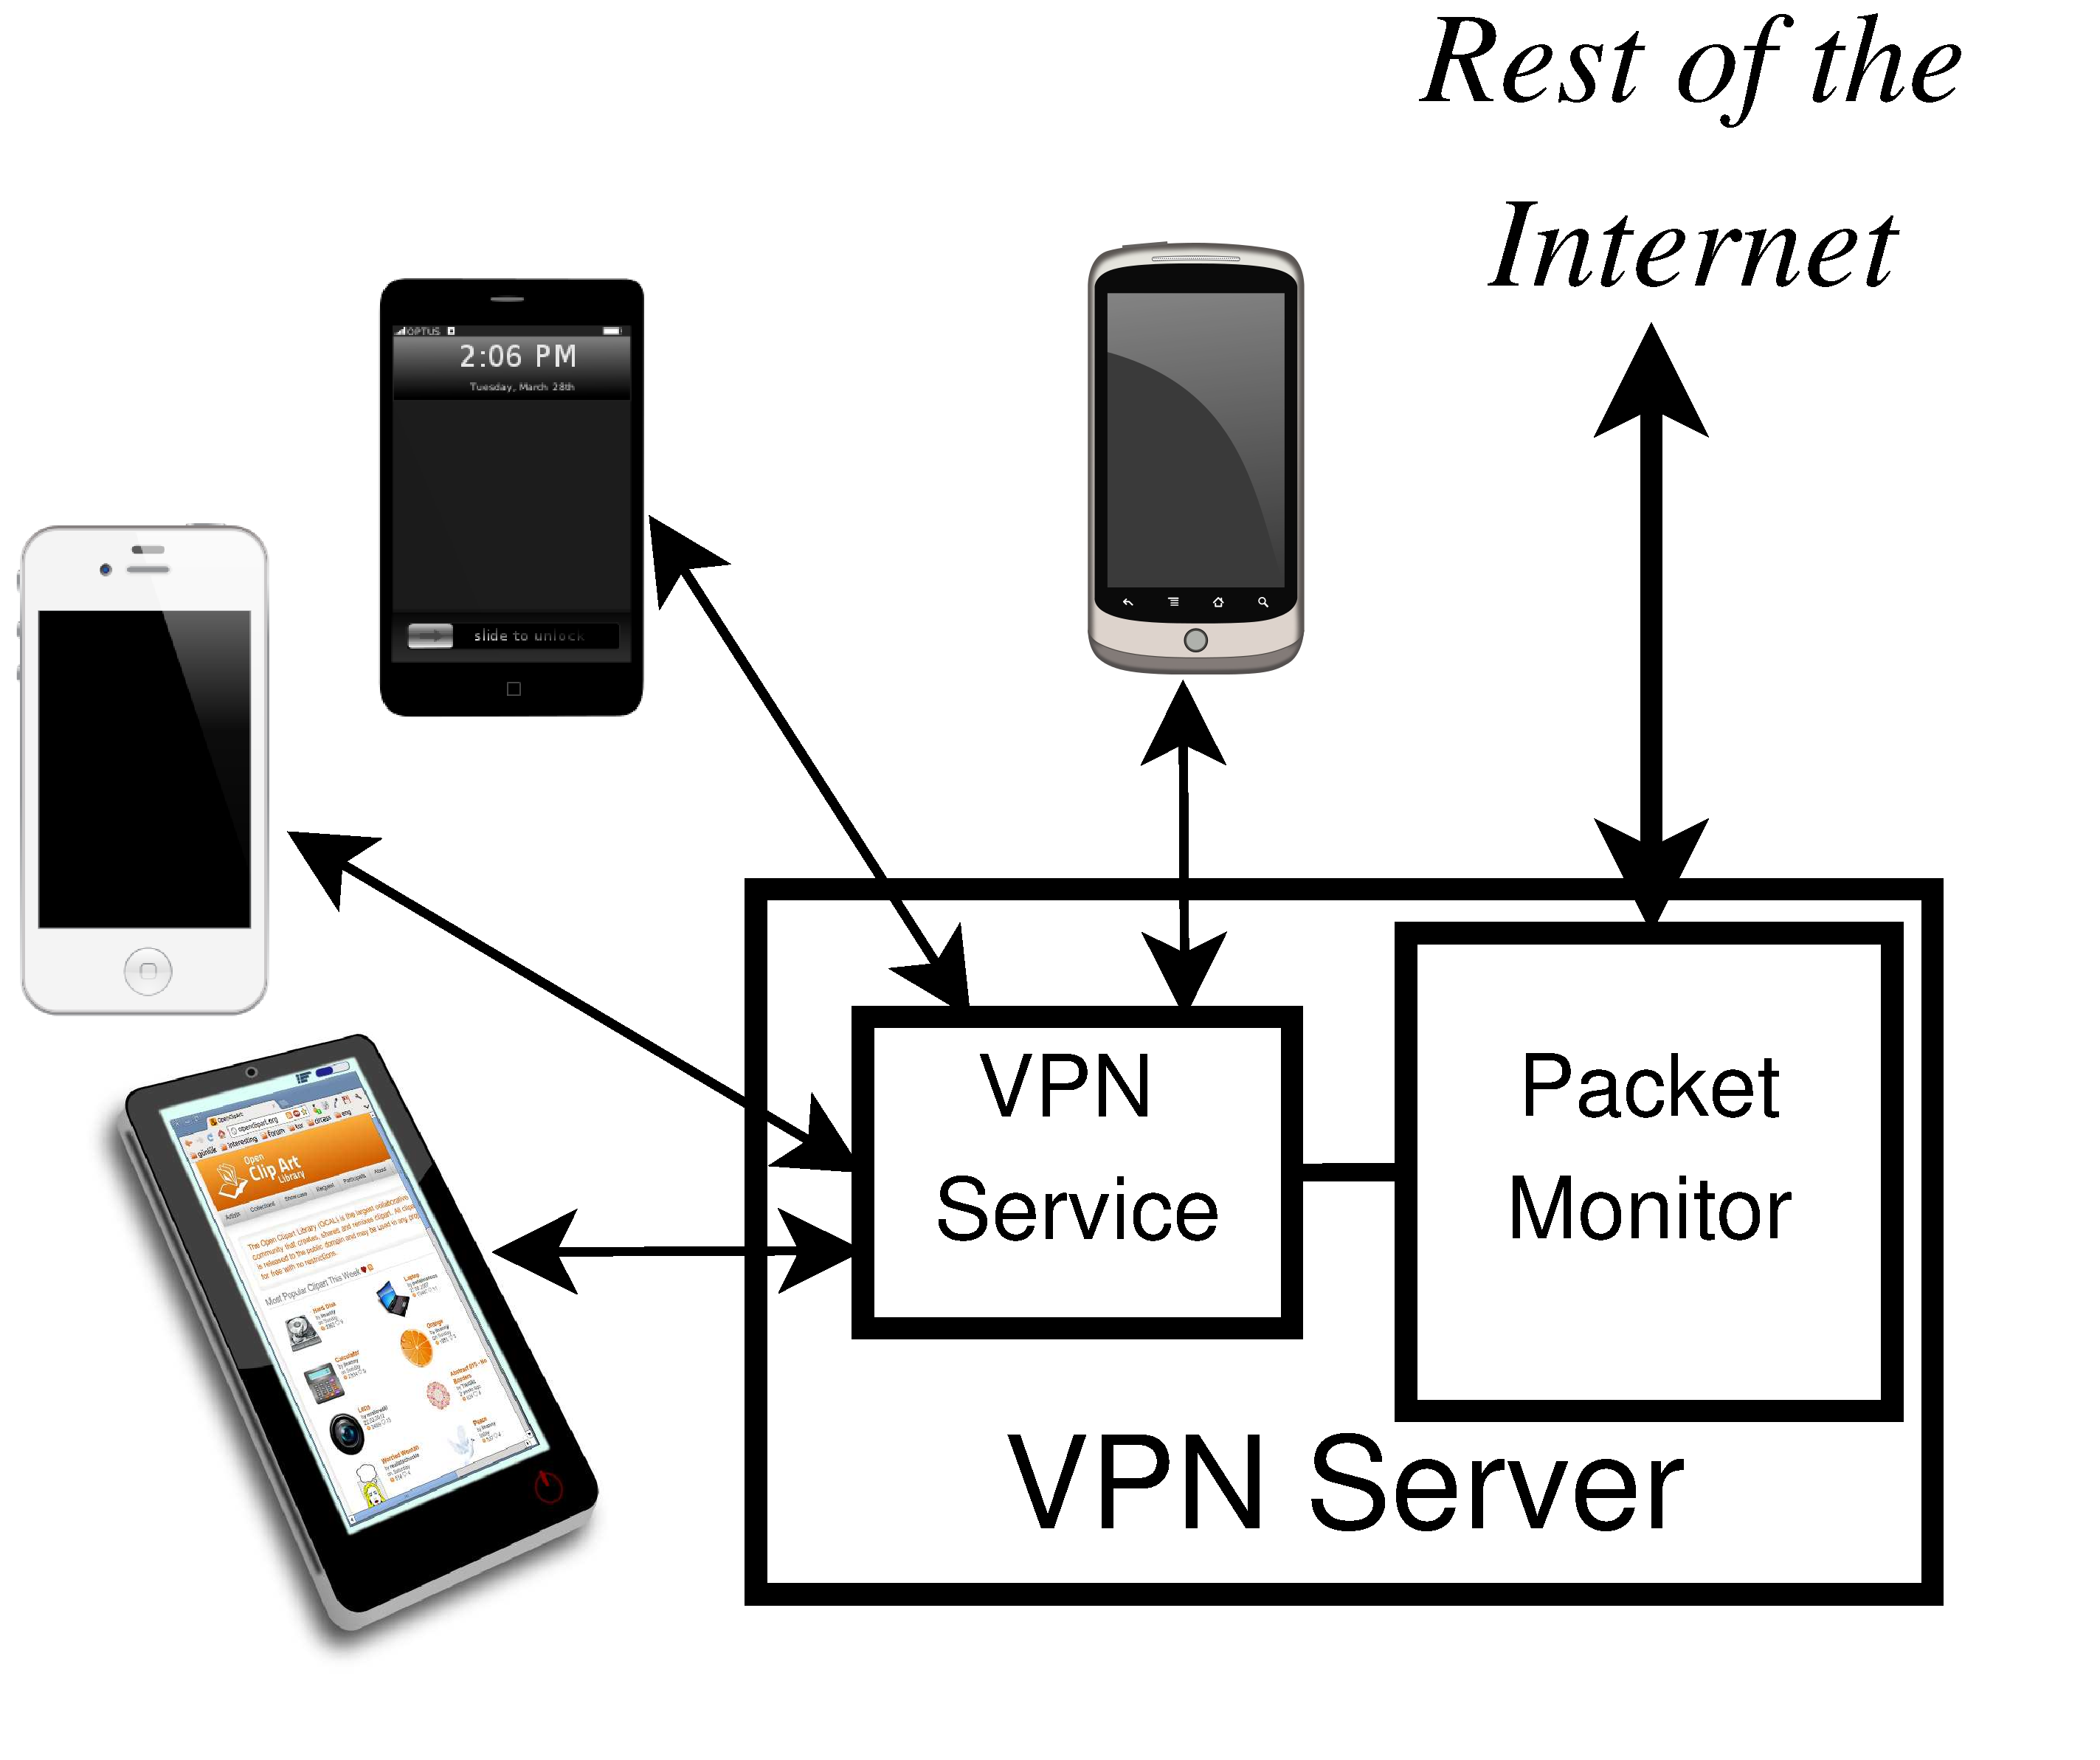
\includegraphics[width=0.75\columnwidth]{figures/meddle-servers.pdf}
%\caption{Hello}
%\label{fig:description}
%\end{figure}

\subsection{Feasibility}

Using trial-and-error, we
discovered that VPN On-Demand uses suffix matching to determine the domains
that require a VPN connection. We use each alphanumeric character as the
set of domains that require a VPN connection. We use this technique to
ensure that a VPN tunnel is created when our iOS devices connect to the
Internet. 


We therefore believe, and show in \ref{sec:feasibility}, that   VPNs to be portable and
deployable. 

We take advantage of the \emph{VPN On-Demand} feature provided by iOS to
ensure that our VPN server is used to tunnel all the mobile traffic from
iOS devices. All iOS devices (version 3.0 and above) come with a feature
called ``VPN On-Demand''. \emph{VPN On-Demand} forces the iOS device to use
VPN tunnels when connecting to a specified set of domains. Using
trial-and-error, we discovered that VPN On-Demand uses suffix matching to
determine the domains that require a VPN connection. We use each
alphanumeric character as the set of domains that require a VPN connection.
We use this technique to ensure that a VPN tunnel is created when our iOS
devices connect to the Internet. 

Android version 4.0 and above comes with native VPN support. Unlike iOS,
Android does not offer an equivalent of \emph{VPN On-Demand}; however,
Android provides an API that allows an user space app to  manage VPN
connections. We modify the open source StrongSwan VPN
client~\cite{strongswanclient} to ensure that the VPN reconnects each time
the preferred network changes (\eg, when a device switches from cellular to
\wifi). As of Android 4.2, Android supports ``Always On'' VPN connections
that uses VPNs to tunnel all the data traffic. \tbd{Text on Issues with Always
ON}.

\section{Feasibility}
\label{sec:feasibility}

\subsubsection{Portable} 
% device, access technology, and service provider. 
Android, BlackBerry, Bada, and iOS all support VPNs natively, representing
more than 86\% of the mobile device market\cite{gartner-phone-share}. These
devices support VPN tunnels over Wi-Fi and the cellular interface.
Furthermore, to satisfy their corporate clients, very few ISPs are known to
block VPN traffic to flow through their networks.  

\subsubsection{Pervasive}
% devices connect seamlessly without periodic action.
We take advantage of the \emph{VPN On-Demand} feature provided by iOS to
ensure that our VPN server is used to tunnel all the mobile traffic from
iOS devices. All iOS devices (version 3.0 and above) come with a feature
called ``VPN On-Demand''. \emph{VPN On-Demand} forces the iOS device to use
VPN tunnels when connecting to a specified set of domains. Using
trial-and-error, we discovered that VPN On-Demand uses suffix matching to
determine the domains that require a VPN connection. We use each
alphanumeric character as the set of domains that require a VPN connection.
We use this technique to ensure that a VPN tunnel is created when our iOS
devices connect to the Internet. 

Android version 4.0 and above comes with native VPN support. Unlike iOS,
Android does not offer an equivalent of \emph{VPN On-Demand}; however,
Android provides an API that allows an user space app to  manage VPN
connections. We modify the open source StrongSwan VPN
client~\cite{strongswanclient} to ensure that the VPN reconnects each time
the preferred network changes (\eg, when a device switches from cellular to
\wifi). As of Android 4.2, Android supports ``Always On'' VPN connections
that uses VPNs to tunnel all the data traffic. \tbd{Text on Issues with Always
ON}.

\subsubsection{Deployable}
% steps to configure tunnel
Manually configuring a VPN generally requires filling out five fields on an
Android phone, and the VPN configuration can be distributed using a single
file on iOS. These configurations are primarily required to drive the key
exchange algorithms that establish the VPN tunnels. This simplicity is
important because it can facilitate large scale measurement studies with
end users.  

%off the shelf hardware and software. need for IPsec. 
Strongswan, Openswan, and OpenVPN are some of the popular VPN daemons that
can be used to manage VPN tunnels. Our platform uses Strongswan because it
is open source and, to the best of our knowledge, it is the only open
source solution that can use the IPsec services of the Linux kernel without
any kernel modifications. IPsec is important because the \emph{VPN
On-Demand} feature of iOS is supported only for VPN tunnels that use IPsec.
Strongswan is supported on vanilla Linux operating systems which ensures
that VPN tunnels can be managed using \emph{off-the-shelf} software and
hardware.


